%------------------------------------------------------------------------------%

\usepackage{apresentacao}
\usepackage{mathconfig}
\usepackage{tabto}

\makeatletter
\graphicspath  {{./figs/}}
\def\input@path{{./figs/}}
\makeatother

%------------------------------------------------------------------------------%
\title {Áreas entre Curvas}
\author{\large Luis Alberto D'Afonseca}
\date  {Integrais e Séries}

%------------------------------------------------------------------------------%
\begin{document}

%------------------------------------------------------------------------------%
\begin{frame}
    \titlepage
\end{frame}

%------------------------------------------------------------------------------%
\section{Áreas entre Curvas}

%------------------------------------------------------------------------------%
\framedgraphic{Área entre Curvas}{area_entre_curvas_01}{}

%------------------------------------------------------------------------------%
\begin{frame}{Definição: Área entre Curvas}
  A área $A$ da região limitada pelas curvas e retas
  \[
    y = f(x)  \qquad
    y = g(x)  \qquad
    x = a     \qquad
    x = b
  \]
  onde $f$ e $g$ são contínuas e
  $f(x) \geq g(x)$ para todo $x \in [a, b]$, é
  \[
    A = \int_a^b f(x) - g(x) \, dx
  \]
\end{frame}

%------------------------------------------------------------------------------%
\section{Exemplo 1}

%------------------------------------------------------------------------------%
\begin{frame}{Exemplo 1}
  Encontre a área da região limitada abaixo por $f(x)= x$, \\
  acima por $g(x)=e^x+1$ e limitada nos lados pelas retas $x=0$ e $x=1$.
\end{frame}

%\framedgraphic{Exemplo 1 -- Interpretação}{areae1}{}
\begin{frame}{Exemplo 1 -- Interpretação}
  \centering
  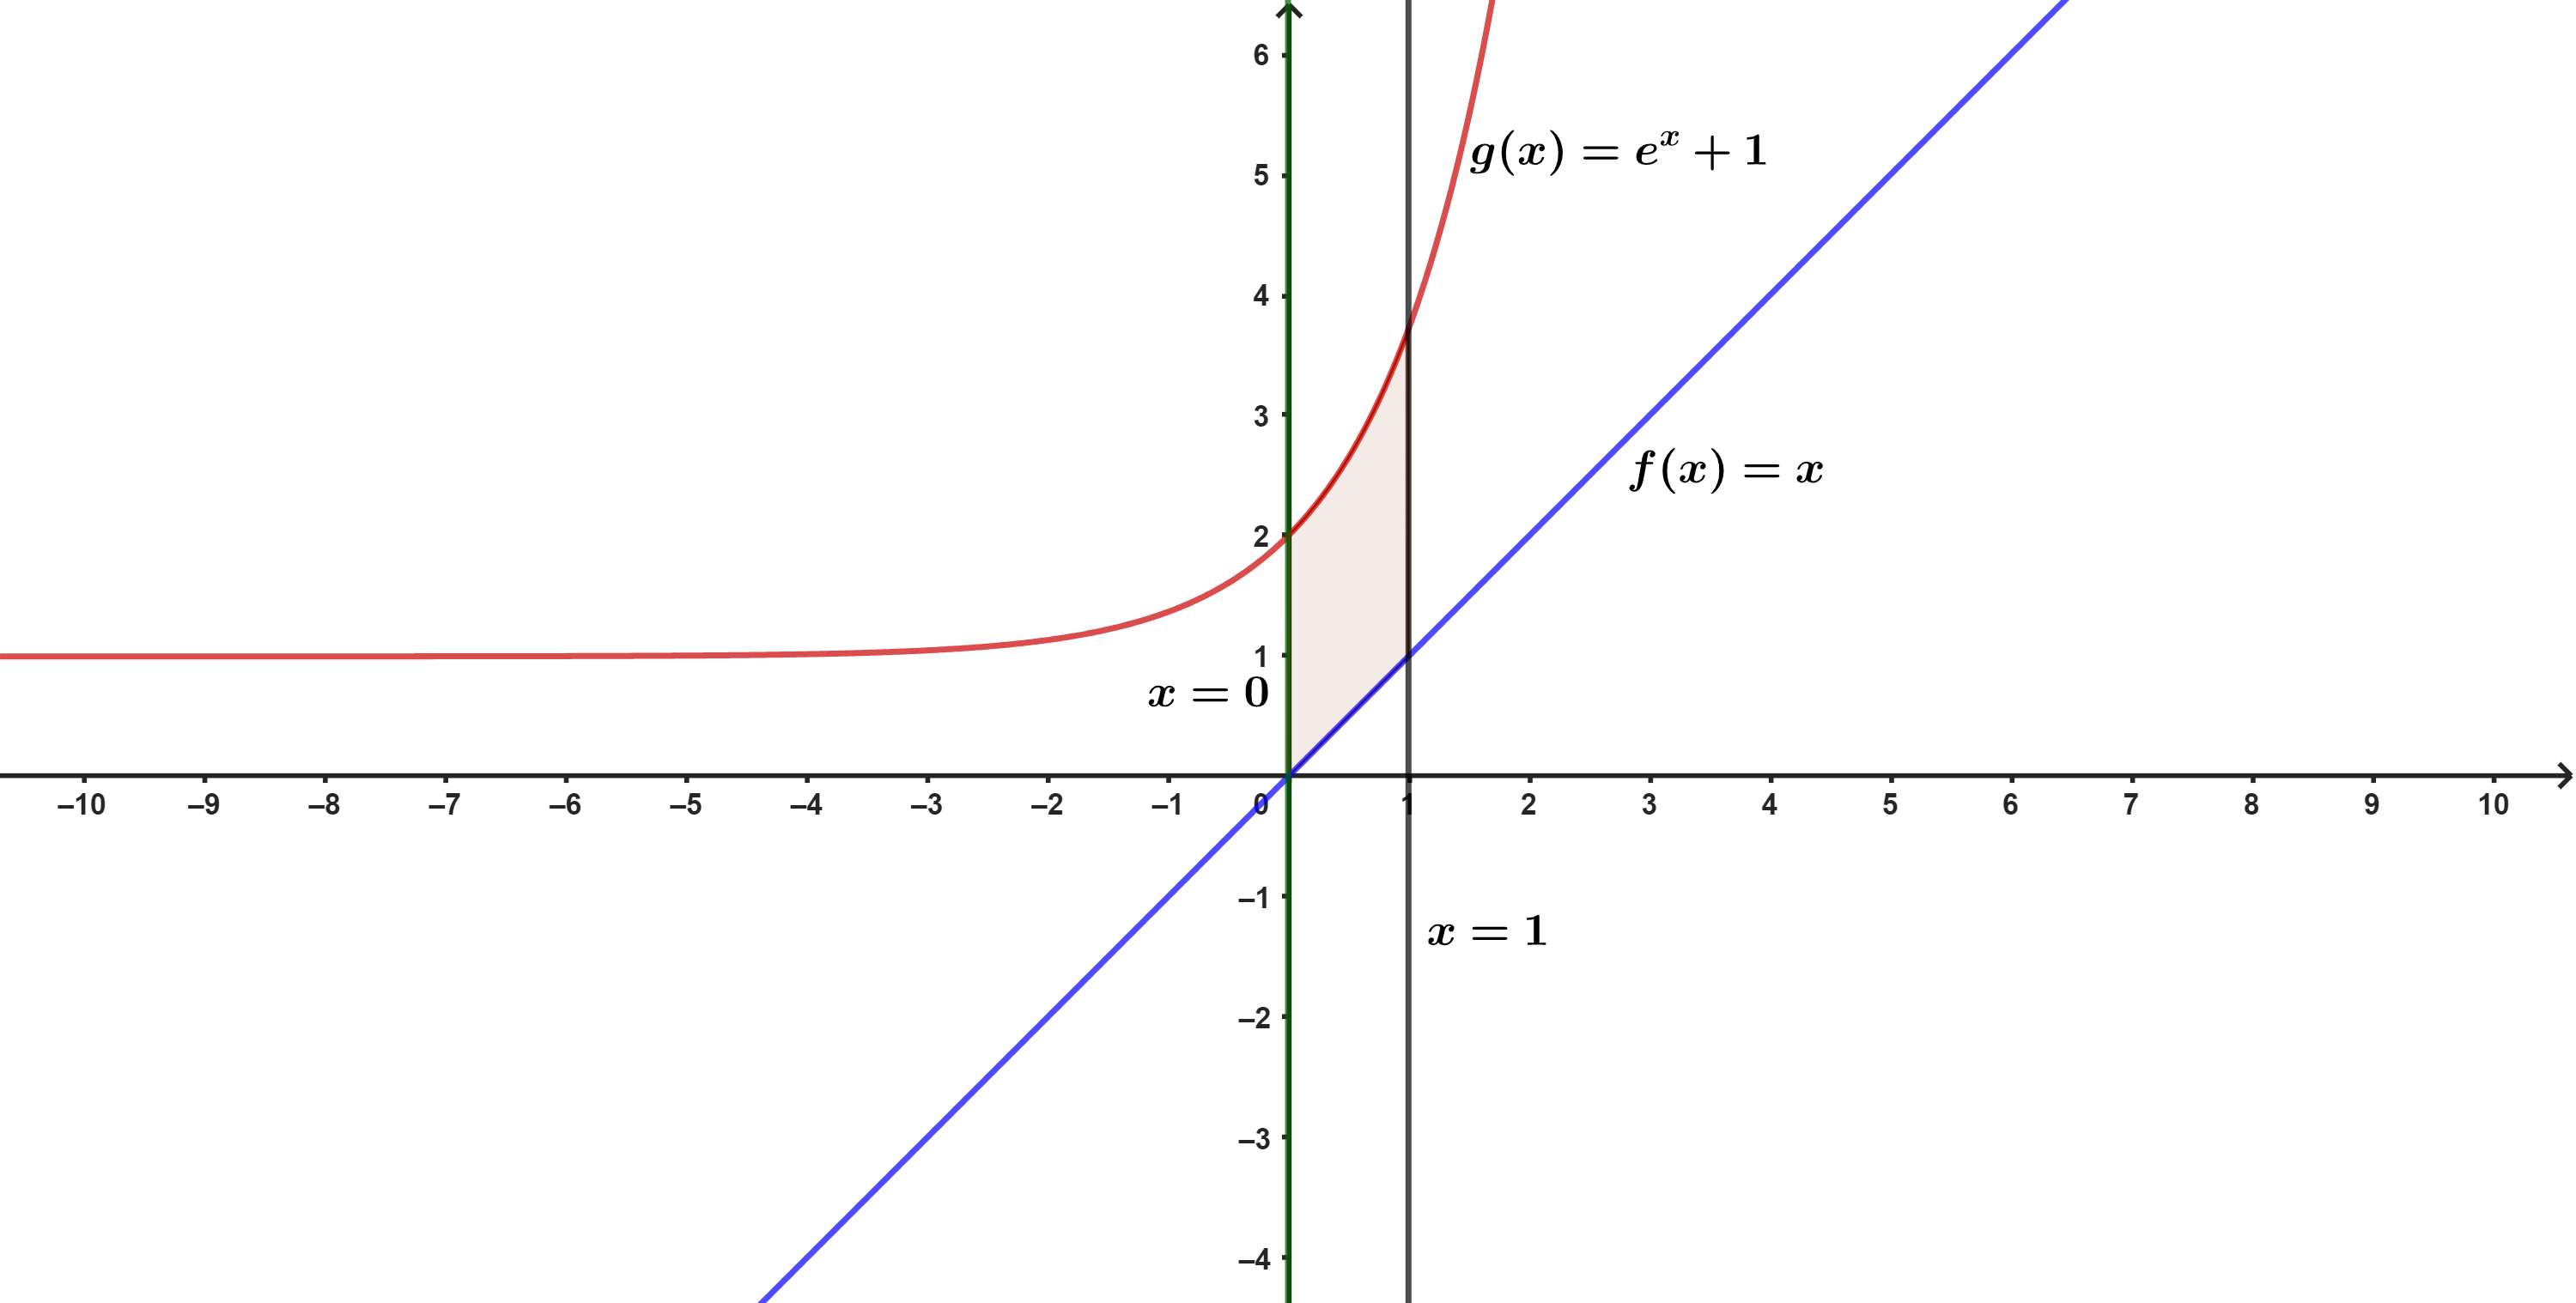
\includegraphics[trim=40mm 28mm 40mm 0mm, clip,
  width=\textwidth,
  height=0.8\textheight,
  keepaspectratio]{areae1}
\end{frame}

\begin{frame}{Exemplo 1 -- Resolução}
  \begin{align*}
    \onslide<+->{ A & = \int_0^1 g(x) - f(x) dx \\[2mm] }
    \onslide<+->{   & = \int_0^1 e^x + 1 - x \, dx \\[2mm]}
    \onslide<+->{   & = \left( e^x+x-\frac{x^2}{2} \right) \evalat{0}{1} & & \text{TFC 2}\\[2mm]}
    \onslide<+->{   & = \left(e+1-\frac{1}{2}\right)-\left(e^0+0-\frac{0}{2}\right) \\[2mm]}
    \onslide<+->{   & = e-\frac{1}{2}}
  \end{align*}
\end{frame}

%------------------------------------------------------------------------------%
\section{Exemplo 2}

%------------------------------------------------------------------------------%
\begin{frame}{Exemplo 2}
  Calcule a área da região delimitada pelas curvas $y = x^2$ e $y = 2x$.
\end{frame}

\begin{frame}{Exemplo 2 -- Interpretação}
  Observe que:
  \begin{itemize}[<+->]
    \setlength\itemsep{1em}
    \item a curva \( y = x^2 \) é uma parábola
    \item a curva \( y = 2x  \) é uma reta que passa pela origem
    \item \( y = 2x  \) está ``por cima''
    \item \( y = x^2 \) está ``por baixo''
    \item os extremos do intervalo precisam ser determinados.
  \end{itemize}
\end{frame}

%\framedgraphic{Exemplo 2 -- Interpretação}{areae2}{}
\begin{frame}{Exemplo 2 -- Interpretação}
  \centering
  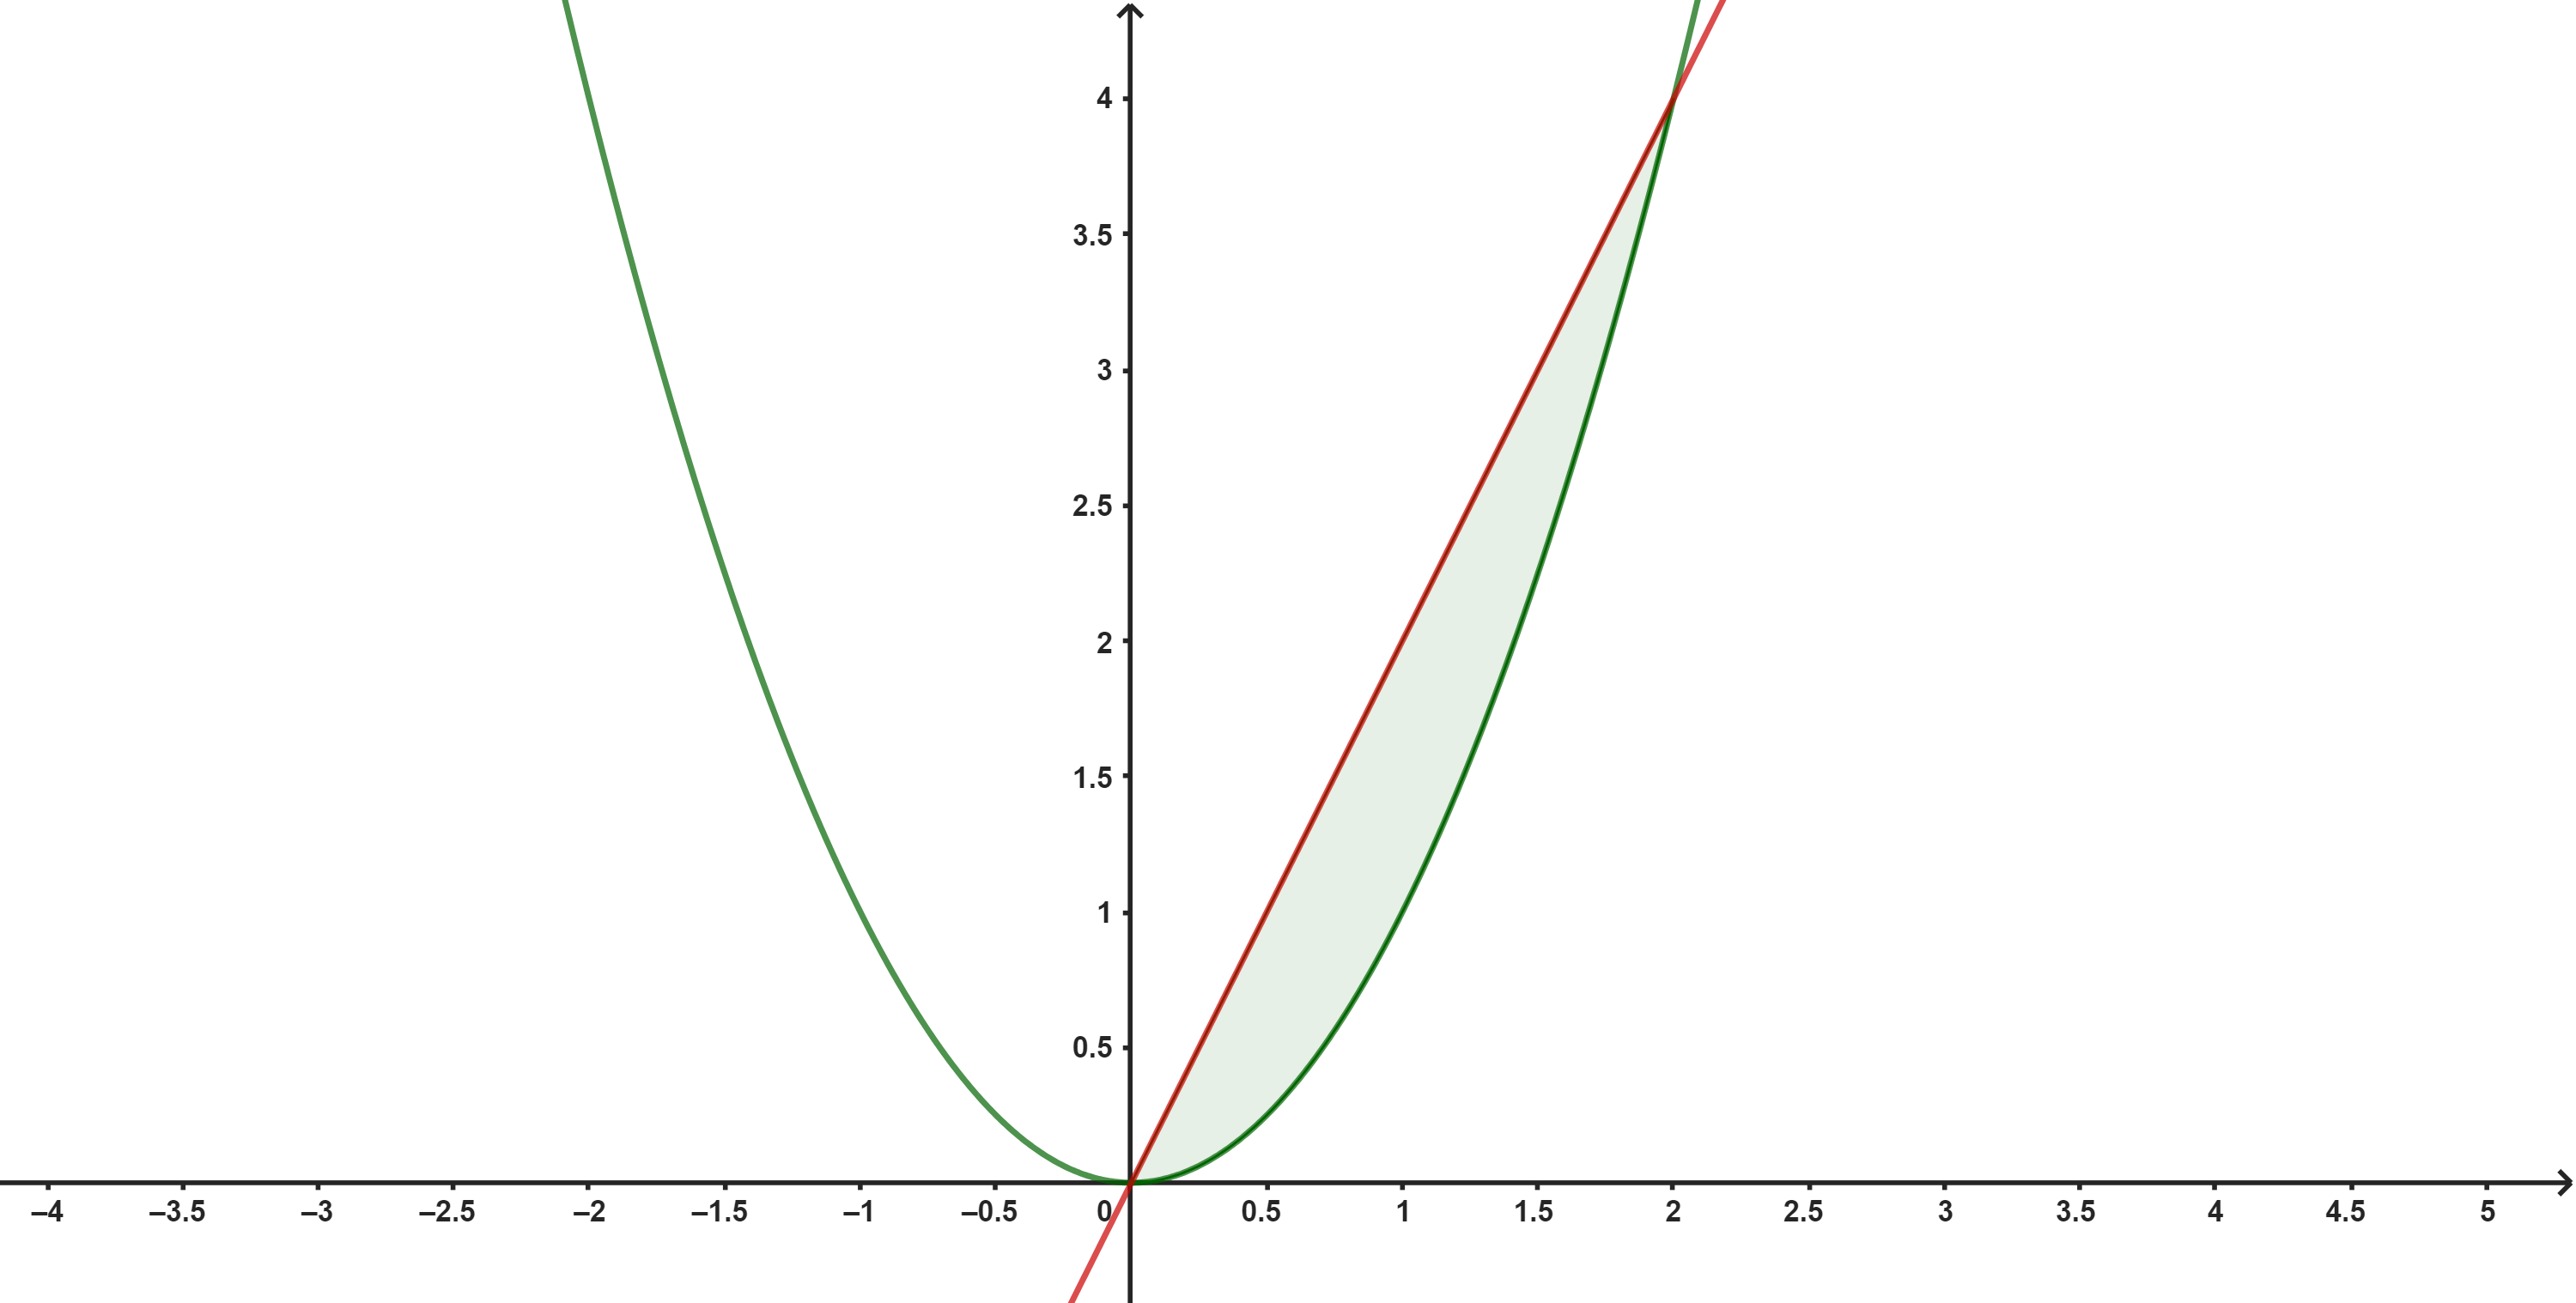
\includegraphics[trim=13mm 0mm 25mm 0mm, clip,
  width=\textwidth,
  height=0.8\textheight]{areae2}
\end{frame}


\begin{frame}{Exemplo 2 -- Resolução}
  Precisamos encontrar os pontos de intersecção das curvas
  \[
    x^2 = 2x
  \]

  \pause
  Soluções: $x=0$ e $x=2$.
\end{frame}

\begin{frame}{Exemplo 2 -- Resolução}
  \begin{align*}
    \onslide<+->{ A & = \int_0^2 2x - x^2 \, dx                                    \\[2mm]}
    \onslide<+->{   & = \left( x^2-\frac{x^3}{3} \right) \evalat{0}{2}             \\[2mm]}
    \onslide<+->{   & = \left( 4- \frac{8}{3}\right) - \left( 0-\frac{0}{3}\right) \\[2mm]}
    \onslide<+->{   & = \frac{4}{3}}
  \end{align*}
\end{frame}

%------------------------------------------------------------------------------%
\section{Exemplo 3}

%------------------------------------------------------------------------------%
\begin{frame}{Exemplo 3}
  Calcular a área da região delimitada pelas curvas
  \[ y = -x^2 + 3x + 2\]
  e
  \[ y = x^2 - 3 \]
\end{frame}

\begin{frame}{Exemplo 3 -- Interpretação}
  Note que, a curva \(y = -x^2 +3x + 2\)
  \begin{itemize}[<+->]
    \setlength\itemsep{1em}
    \item é uma parábola com concavidade voltada para baixo
    \item seu vértice é
          \(
            \left(\frac{-b}{2a}, \frac{-\Delta}{4a}\right) =
            \left(\frac{3}{2}, \frac{17}{4}\right)
          \)
    \item suas raízes são
          \(
            x_1 = \frac{3+\sqrt{17}}{2}
            \qquad
            x_2 = \frac{3-\sqrt{17}}{2}
          \)
    \item intercepta o eixo $y$ no ponto $(0, 2)$
  \end{itemize}
\end{frame}

\begin{frame}{Exemplo 3 -- Interpretação}
  Enquanto a curva \(y = x^2 - 3\)
  \begin{itemize}[<+->]
    \setlength\itemsep{1em}
    \item é uma parábola com concavidade voltada para cima
    \item seu vértice é $(0, -3)$
    \item suas raízes são $x_1 = \sqrt{3}$ e $x_2 = -\sqrt{3}$
    \item intercepta o eixo $y$ no ponto $(0, -3)$
  \end{itemize}
\end{frame}

%\framedgraphic{Exemplo 3 -- Interpretação}{areae3}{}
\begin{frame}{Exemplo 3 -- Interpretação}
  \centering
  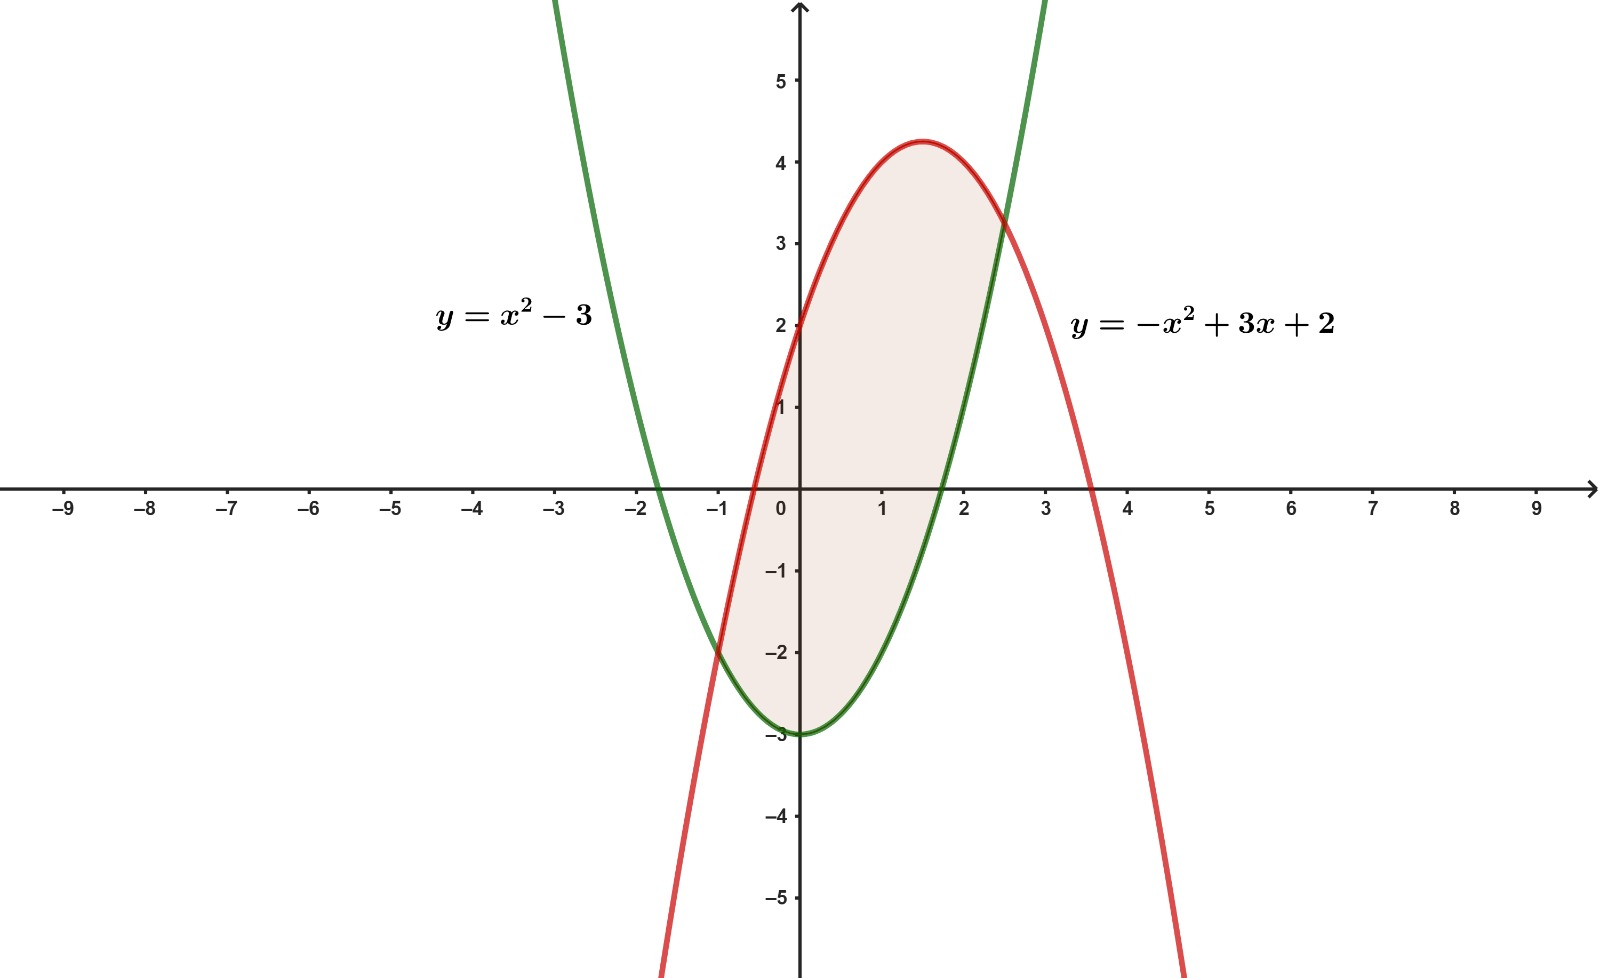
\includegraphics[trim=40mm 10mm 40mm 0mm, clip,
  width=\textwidth,
  height=0.8\textheight,
  keepaspectratio]{area_exemplo_3}
\end{frame}

\begin{frame}{Exemplo 3 -- Resolução}
  Pontos de intersecção
  \[
    -x^2 +3x + 2 = x^2 - 3
  \]
  Soluções: \(x = -1\) e \(x = \frac{5}{2}\)
\end{frame}

\begin{frame}{Exemplo 3 -- Resolução}
  \begin{align*}
    \onslide<+->{
      A
      & = \int_{-1}^{\sfrac{5}{2}} \left(-x^2 + 3x +  2\right) - \left( x^2 -3 \right) \, dx \\[2mm]}
    \onslide<+->{
      & = \int_{-1}^{\sfrac{5}{2}} -2x^2 +3x + 5  \, dx  \\[2mm]}
    \onslide<+->{
      & = \left( -\frac{2}{3}x^3 -\frac{3}{2}x^2 +5x \right) \evalat{-1}{\sfrac{5}{2}} \\[2mm]}
    \onslide<+->{
      & = \left(
        - \frac{2}{3} \frac{125}{8}
        + \frac{3}{2} \frac{25}{4}
        + 5 \frac{5}{2}
      \right)
      - \left(
        - \frac{2}{3} (-1)^3
        + \frac{3}{2} (-1)^2
        + 5 (-1)
      \right) \\[2mm]}
      \onslide<+->{
      & = \frac{343}{24}}
  \end{align*}
\end{frame}

%------------------------------------------------------------------------------%
\section{Exemplo 4}

%------------------------------------------------------------------------------%
\begin{frame}{Exemplo 4}
  Calcule a área da região delimitada pelas curvas
  \[
    f(x) = \sin(x)
    \quad\text{e}\quad
    g(x) = \cos(x)
  \]
  no intervalo
  \([0, \sfrac{\pi}{2}]\)
\end{frame}

\begin{frame}{Exemplo 4 -- Interpretação}
  \begin{itemize}[<+->]
    \setlength\itemsep{1em}
    \item pontos de interseção
          \[ \sin(x) = \cos(x) \qquad 0 \leq x \leq \sfrac{\pi}{2} \]
          \[ x = \sfrac{\pi}{4} \]

    \item pelo gráfico podemos notar que
          \[\cos(x) \geq \sin(x) \qquad 0 \leq x \leq \sfrac{\pi}{4} \]
          \[\sin(x) \geq \cos(x) \qquad \sfrac{\pi}{4} \leq x \leq \sfrac{\pi}{2} \]

    \item precisamos dividir a região em duas partes
  \end{itemize}
\end{frame}

\framedgraphic{Exemplo 4 -- Interpretação}{areae4}{}

\begin{frame}{Exemplo 4 -- Resolução}
  \begin{align*}
    \onslide<+->{A & = A_1 + A_2                                                                 \\[2mm]}
    \onslide<+->{  & = \int_0^{\sfrac{\pi}{4}}                \cos(x) - \sin(x) \,dx
                     + \int_{\sfrac{\pi}{4}}^{\sfrac{\pi}{2}} \sin(x) - \cos(x) \,dx             \\[2mm]}
    \onslide<+->{  & = \big(  \sin(x) + \cos(x) \big) \evalat{0}{\sfrac{\pi}{4}}
                     + \big( -\cos(x) - \sin(x) \big) \evalat{\sfrac{\pi}{4}}{\sfrac{\pi}{2}}    \\[2mm]}
    \onslide<+->{  & = \left( \frac{\sqrt{2}}{2} + \frac{\sqrt{2}}{2} -0 -1 \right)
                     + \left( -0 -1 + \frac{\sqrt{2}}{2} + \frac{\sqrt{2}}{2} \right)            \\[2mm]}
    \onslide<+->{  & = 2\sqrt{2}-2}
  \end{align*}
\end{frame}


\begin{frame}{Simetrias}
  Poderíamos ter aproveitado a
  simetria da região em relação à reta $x = \sfrac{\pi}{4}$,
  o que nos permitiria economizar esforço ao calcular a área, uma vez que
  \[
    A
    = 2 A_1
    = 2 \int_0^{\sfrac{\pi}{4}} \cos(x) - \sin(x) \,dx
  \]
\end{frame}

%------------------------------------------------------------------------------%
\section{Exemplo 5}

%------------------------------------------------------------------------------%
\begin{frame}{Exemplo 5}
  Calcule a área da região expressa na figura, que é uma das regiões
  delimitada simultaneamente pelas três curvas
  \[
    f(x) = 2x-1, \qquad
    g(x) =-\frac{x}{2}+4\quad\text{e}\quad
    h(x)=(x-2)^2
  \]
  \centerline{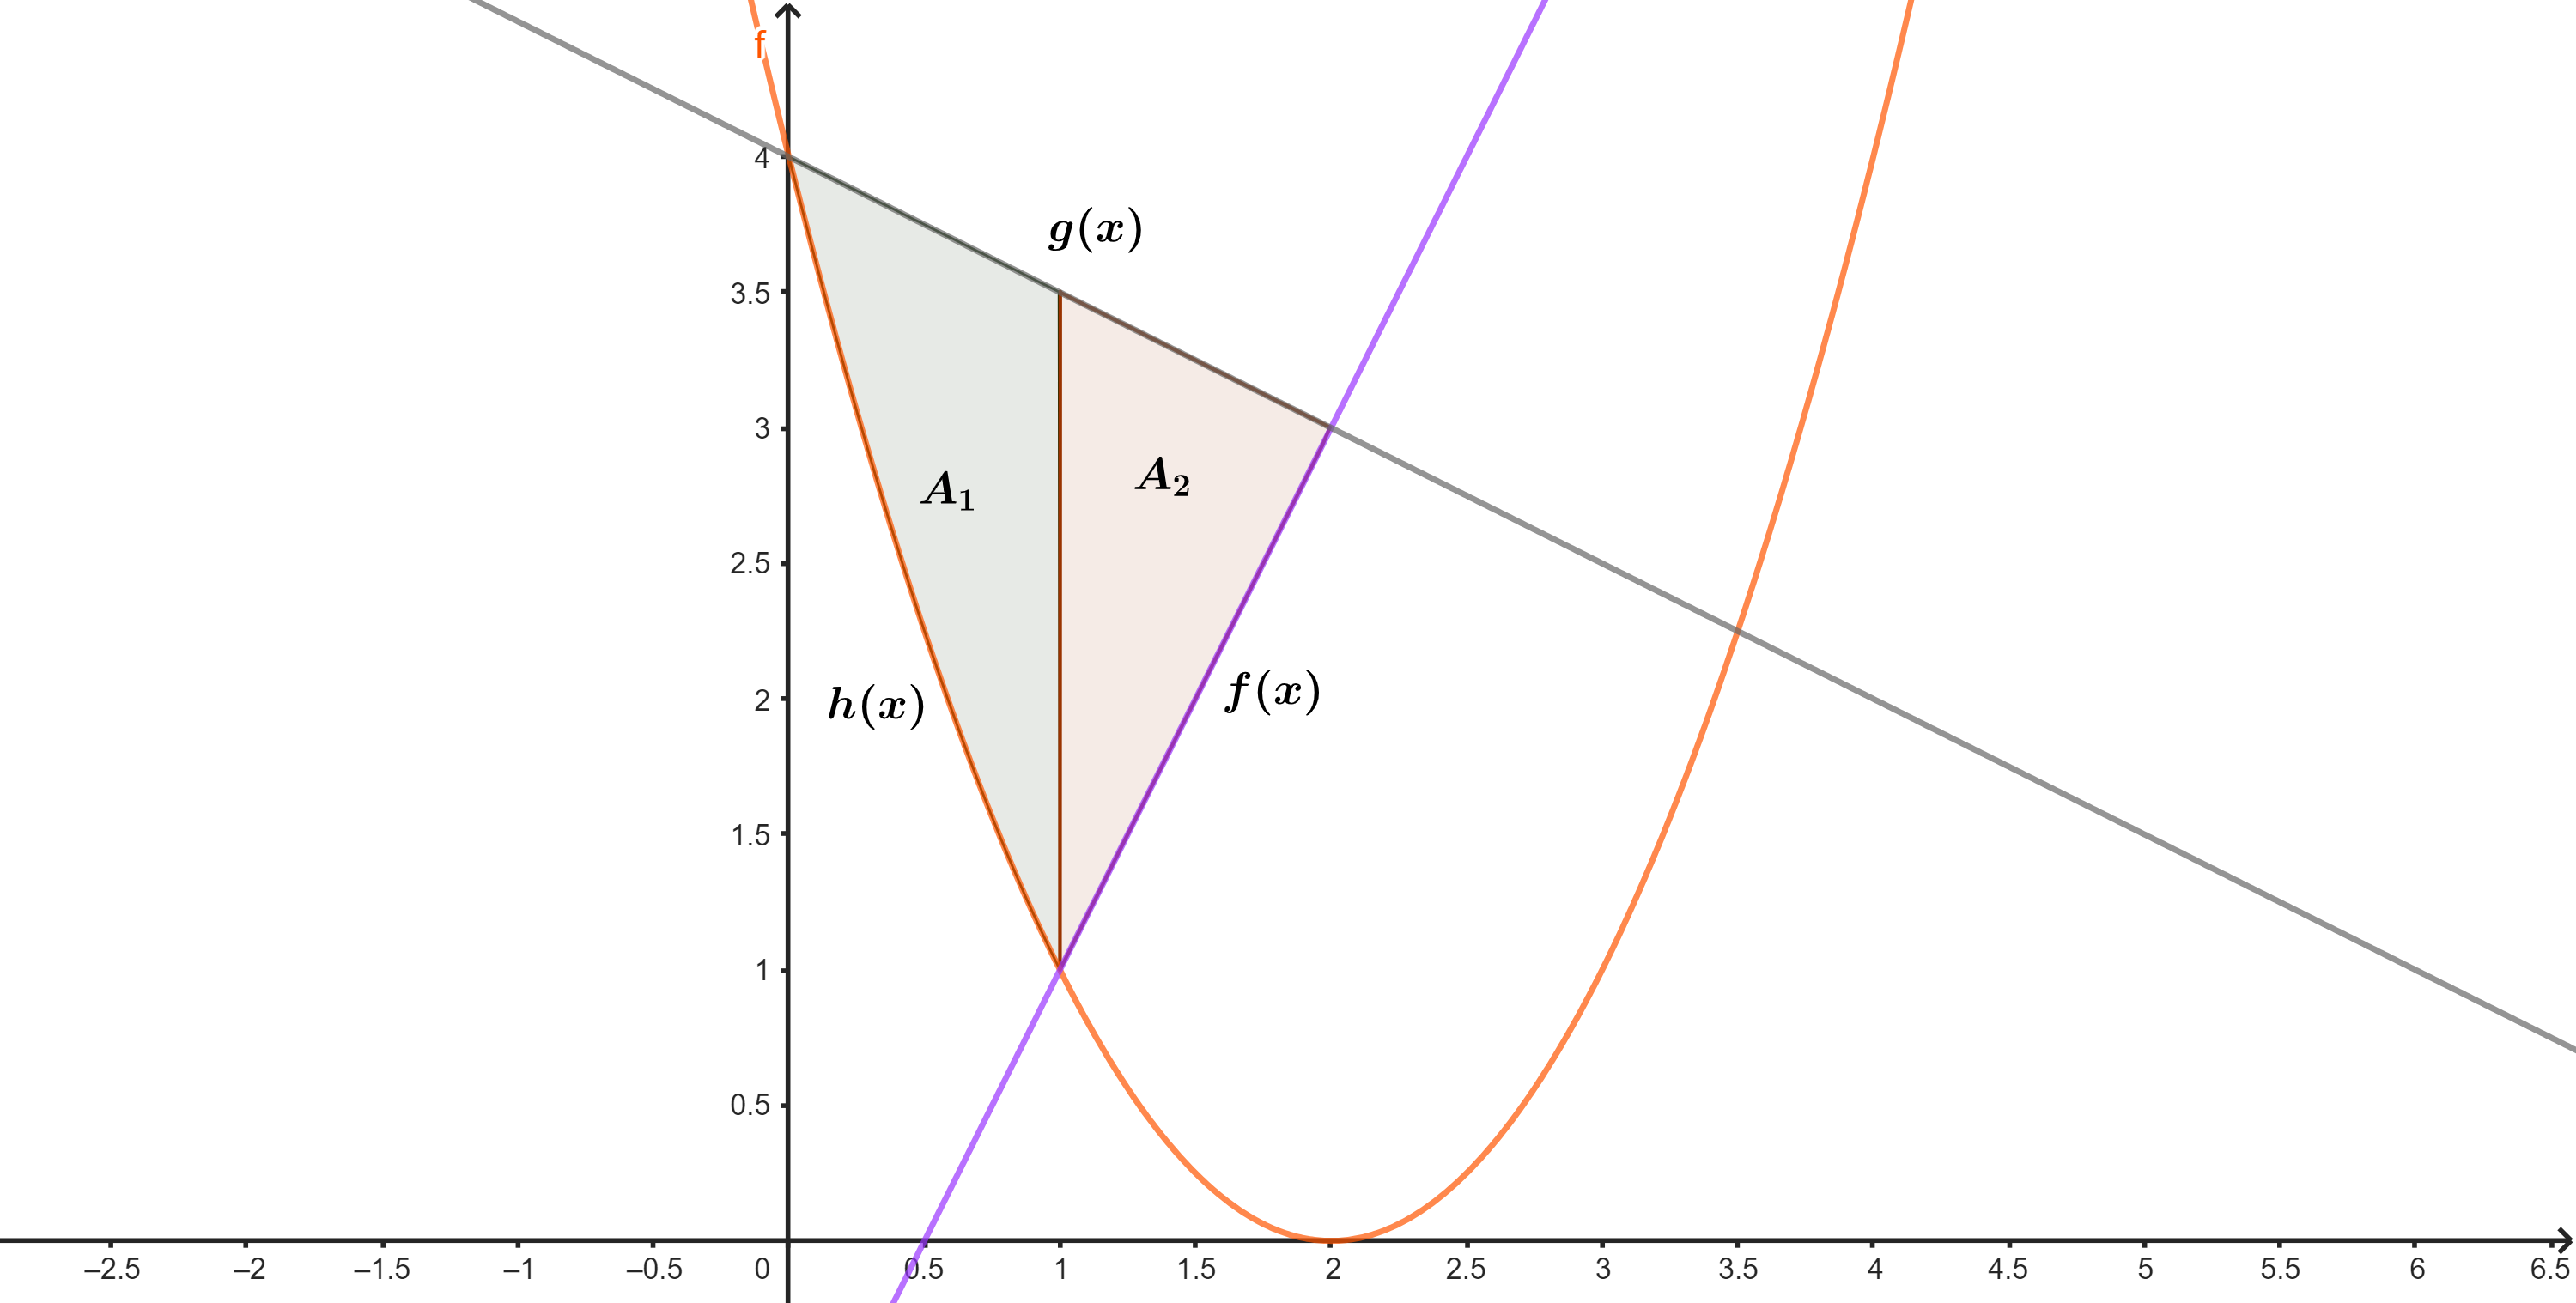
\includegraphics[height=50mm]{areae51}}
\end{frame}

\begin{frame}{Exemplo 5 -- Interpretação}
  \begin{itemize}[<+->]
    \setlength\itemsep{1em}
    \item $f(x)$ e $g(x)$ são retas
    \item \(h(x)=(x-2)^2=x^2-4x+4\) é parábola com concavidade para cima
    \item vértice $(2, 0)$
    \item raiz $x = 2$
  \end{itemize}
\end{frame}

\begin{frame}{Exemplo 5 -- Interpretação}
  \begin{itemize}[<+->]
    \setlength\itemsep{1em}
    \item precisamos dividir a região em duas
    \item Na primeira, de 0 até 1                                   \\[2mm]
          \(g(x) = -\sfrac{x}{2}+4\) \tabto{37mm} está ``por cima'' \\[2mm]
          \(h(x) = (x-2)^2\)         \tabto{37mm} está ``por baixo''
    \item Na segunda, de 1 até 2                                    \\[2mm]
          \(g(x) = -\sfrac{x}{2}+4\) \tabto{37mm} está ``por cima'' \\[2mm]
          \(f(x) = 2x-1\)            \tabto{37mm} está ``por baixo''
  \end{itemize}
\end{frame}

\begin{frame}{Exemplo 5 -- Resolução}
  \begin{align*}
    \onslide<+->{A_1 & = \int_0^1 g(x) - h(x) dx \\[5mm]}
    \onslide<+->{A_2 & = \int_1^2 g(x) - f(x) dx}
  \end{align*}
\end{frame}

\begin{frame}{Exemplo 5 -- Resolução}
  \begin{align*}
    \onslide<+->{A_1 & = \int_0^1 \left(-\frac{x}{2}+4\right) - \left(x^2-4x+4\right) \, dx \\[2mm]}
    \onslide<+->{    & = \int_0^1 -x^2 + \frac{7}{2}x \,  dx                        \\[2mm]}
    \onslide<+->{    & = \left( -\frac{x^3}{3}+\frac{7}{4}x^2 \right) \evalat{0}{1} \\[2mm]}
    \onslide<+->{    & = \left(-\frac{1}{3}+\frac{7}{4} \right)-(0-0)               \\[2mm]}
    \onslide<+->{    & = \frac{17}{12}}
  \end{align*}
\end{frame}

\begin{frame}{Exemplo 5 -- Resolução}
  \begin{align*}
    \onslide<+->{A_2 & = \int_1^2 \left(-\frac{x}{2}+4\right)-\left(2x-1\right) \, dx                      \\[2mm]}
    \onslide<+->{    & = \int_1^2 -\frac{5x}{2}+5 \, dx                              \\[2mm]}
    \onslide<+->{    & = \left( -\frac{5x^2}{4}+5x \right) \evalat{1}{2}             \\[2mm]}
    \onslide<+->{    & = \left(-\frac{20}{4}+10 \right)-\left(-\frac{5}{4}+5 \right) \\[2mm]}
    \onslide<+->{    & = \frac{5}{4}}
  \end{align*}
\end{frame}

\begin{frame}{Exemplo 5 -- Resolução}
  \[
    A
    = A_1 + A_2
    \pause
    = \frac{17}{12} + \frac{5}{4}
    \pause
    = \frac{8}{3}
  \]
\end{frame}

%------------------------------------------------------------------------------%
\begin{frame}
  \tableofcontents
\end{frame}

%------------------------------------------------------------------------------%
\end{document}
%------------------------------------------------------------------------------%
